\section*{Introducción}
En este número os vamos a hablar de polinomios: polinomios de una variable con coeficientes reales. Sea el polinomio $p(x)$ de grado $n$ dado como sigue en la ecuación (\ref{eq:poln}),
\begin{equation}\label{eq:poln}
P(x)=a_n x^n + a_{n-1}x^{n-1}+\dots+a_{1}x+a_{0},
\end{equation}
donde $n\in \mathbb{N}$, y $a_i\in\mathbb{R}$ con $i\in \{0,1,2,...,n\}$. El término $a_n$ debe ser distinto de cero y se denomina coeficiente director de $P(x)$ y $n$ el grado del polinomio.

En Octave los polinomios se representan  matricialmente como un vector fila. De este modo el polinomio dado en la ecuacion (\ref{eq:poln}) se representa en Octave con el vector fila siguiente: $[a_n\: a_{n-1}\: \dots \:a_1 \:a_0]$. Por ejemplo el polinomio $3x^3+2x+1$ es representado en Octave como el vector fila $[3\: 0\: 2\: 1]$. Veamos el gráfico de algunos polinomios en la Figura \ref{fig:polis}.
\begin{figure}[ht!]
  \centering
  \begin{figurebox}
  \centering
%\begin{figure}
%  \centering
    \scalebox{0.7}{% Title: glps_renderer figure
% Creator: GL2PS 1.3.8, (C) 1999-2012 C. Geuzaine
% For: Octave
% CreationDate: Tue May 13 08:35:53 2014
\setlength{\unitlength}{1pt}
\begin{picture}(0,0)
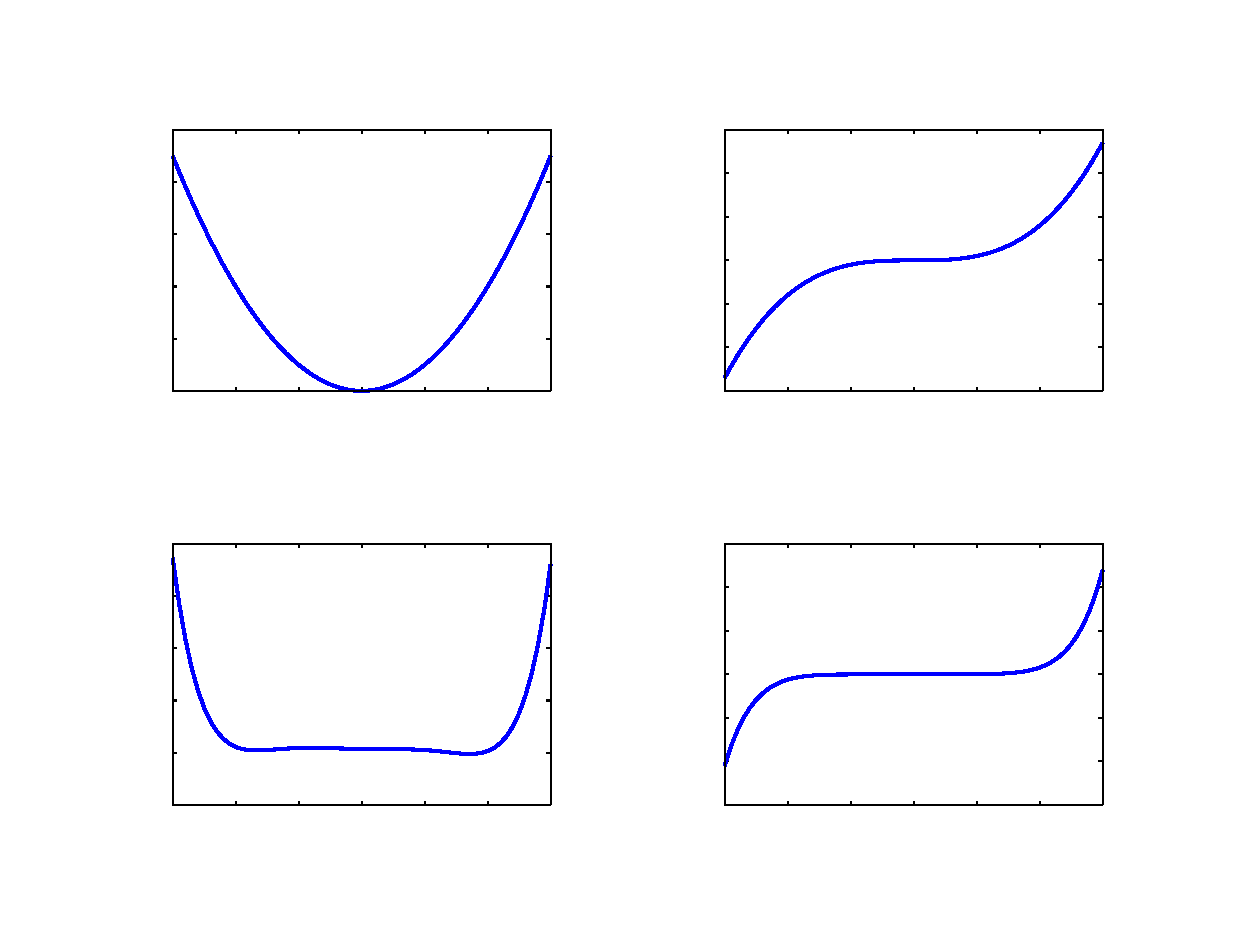
\includegraphics{grafplotB-inc}
\end{picture}%
\begin{picture}(576,432)(0,0)
\fontsize{10}{0}
\selectfont\put(74.88,247.207){\makebox(0,0)[t]{\textcolor[rgb]{0,0,0}{{-3}}}}
\fontsize{10}{0}
\selectfont\put(105.12,247.207){\makebox(0,0)[t]{\textcolor[rgb]{0,0,0}{{-2}}}}
\fontsize{10}{0}
\selectfont\put(135.36,247.207){\makebox(0,0)[t]{\textcolor[rgb]{0,0,0}{{-1}}}}
\fontsize{10}{0}
\selectfont\put(165.6,247.207){\makebox(0,0)[t]{\textcolor[rgb]{0,0,0}{{0}}}}
\fontsize{10}{0}
\selectfont\put(195.84,247.207){\makebox(0,0)[t]{\textcolor[rgb]{0,0,0}{{1}}}}
\fontsize{10}{0}
\selectfont\put(226.08,247.207){\makebox(0,0)[t]{\textcolor[rgb]{0,0,0}{{2}}}}
\fontsize{10}{0}
\selectfont\put(256.32,247.207){\makebox(0,0)[t]{\textcolor[rgb]{0,0,0}{{3}}}}
\fontsize{10}{0}
\selectfont\put(69.8678,252.218){\makebox(0,0)[r]{\textcolor[rgb]{0,0,0}{{0}}}}
\fontsize{10}{0}
\selectfont\put(69.8678,277.271){\makebox(0,0)[r]{\textcolor[rgb]{0,0,0}{{2}}}}
\fontsize{10}{0}
\selectfont\put(69.8678,302.325){\makebox(0,0)[r]{\textcolor[rgb]{0,0,0}{{4}}}}
\fontsize{10}{0}
\selectfont\put(69.8678,327.379){\makebox(0,0)[r]{\textcolor[rgb]{0,0,0}{{6}}}}
\fontsize{10}{0}
\selectfont\put(69.8678,352.432){\makebox(0,0)[r]{\textcolor[rgb]{0,0,0}{{8}}}}
\fontsize{10}{0}
\selectfont\put(69.8678,377.486){\makebox(0,0)[r]{\textcolor[rgb]{0,0,0}{{10}}}}
\fontsize{10}{0}
\selectfont\put(165.6,387.486){\makebox(0,0)[b]{\textcolor[rgb]{0,0,0}{{$p_1(x)=x^2$}}}}
\fontsize{10}{0}
\selectfont\put(339.84,247.207){\makebox(0,0)[t]{\textcolor[rgb]{0,0,0}{{-3}}}}
\fontsize{10}{0}
\selectfont\put(370.08,247.207){\makebox(0,0)[t]{\textcolor[rgb]{0,0,0}{{-2}}}}
\fontsize{10}{0}
\selectfont\put(400.32,247.207){\makebox(0,0)[t]{\textcolor[rgb]{0,0,0}{{-1}}}}
\fontsize{10}{0}
\selectfont\put(430.56,247.207){\makebox(0,0)[t]{\textcolor[rgb]{0,0,0}{{0}}}}
\fontsize{10}{0}
\selectfont\put(460.8,247.207){\makebox(0,0)[t]{\textcolor[rgb]{0,0,0}{{1}}}}
\fontsize{10}{0}
\selectfont\put(491.04,247.207){\makebox(0,0)[t]{\textcolor[rgb]{0,0,0}{{2}}}}
\fontsize{10}{0}
\selectfont\put(521.28,247.207){\makebox(0,0)[t]{\textcolor[rgb]{0,0,0}{{3}}}}
\fontsize{10}{0}
\selectfont\put(334.828,252.218){\makebox(0,0)[r]{\textcolor[rgb]{0,0,0}{{-30}}}}
\fontsize{10}{0}
\selectfont\put(334.828,273.096){\makebox(0,0)[r]{\textcolor[rgb]{0,0,0}{{-20}}}}
\fontsize{10}{0}
\selectfont\put(334.828,293.974){\makebox(0,0)[r]{\textcolor[rgb]{0,0,0}{{-10}}}}
\fontsize{10}{0}
\selectfont\put(334.828,314.852){\makebox(0,0)[r]{\textcolor[rgb]{0,0,0}{{0}}}}
\fontsize{10}{0}
\selectfont\put(334.828,335.73){\makebox(0,0)[r]{\textcolor[rgb]{0,0,0}{{10}}}}
\fontsize{10}{0}
\selectfont\put(334.828,356.608){\makebox(0,0)[r]{\textcolor[rgb]{0,0,0}{{20}}}}
\fontsize{10}{0}
\selectfont\put(334.828,377.486){\makebox(0,0)[r]{\textcolor[rgb]{0,0,0}{{30}}}}
\fontsize{10}{0}
\selectfont\put(430.56,387.486){\makebox(0,0)[b]{\textcolor[rgb]{0,0,0}{{$p_2(x)=x^3$}}}}
\fontsize{10}{0}
\selectfont\put(74.88,48.4869){\makebox(0,0)[t]{\textcolor[rgb]{0,0,0}{{-3}}}}
\fontsize{10}{0}
\selectfont\put(105.12,48.4869){\makebox(0,0)[t]{\textcolor[rgb]{0,0,0}{{-2}}}}
\fontsize{10}{0}
\selectfont\put(135.36,48.4869){\makebox(0,0)[t]{\textcolor[rgb]{0,0,0}{{-1}}}}
\fontsize{10}{0}
\selectfont\put(165.6,48.4869){\makebox(0,0)[t]{\textcolor[rgb]{0,0,0}{{0}}}}
\fontsize{10}{0}
\selectfont\put(195.84,48.4869){\makebox(0,0)[t]{\textcolor[rgb]{0,0,0}{{1}}}}
\fontsize{10}{0}
\selectfont\put(226.08,48.4869){\makebox(0,0)[t]{\textcolor[rgb]{0,0,0}{{2}}}}
\fontsize{10}{0}
\selectfont\put(256.32,48.4869){\makebox(0,0)[t]{\textcolor[rgb]{0,0,0}{{3}}}}
\fontsize{10}{0}
\selectfont\put(69.8678,53.4977){\makebox(0,0)[r]{\textcolor[rgb]{0,0,0}{{-100}}}}
\fontsize{10}{0}
\selectfont\put(69.8678,78.5513){\makebox(0,0)[r]{\textcolor[rgb]{0,0,0}{{0}}}}
\fontsize{10}{0}
\selectfont\put(69.8678,103.605){\makebox(0,0)[r]{\textcolor[rgb]{0,0,0}{{100}}}}
\fontsize{10}{0}
\selectfont\put(69.8678,128.658){\makebox(0,0)[r]{\textcolor[rgb]{0,0,0}{{200}}}}
\fontsize{10}{0}
\selectfont\put(69.8678,153.712){\makebox(0,0)[r]{\textcolor[rgb]{0,0,0}{{300}}}}
\fontsize{10}{0}
\selectfont\put(69.8678,178.766){\makebox(0,0)[r]{\textcolor[rgb]{0,0,0}{{400}}}}
\fontsize{10}{0}
\selectfont\put(165.6,188.766){\makebox(0,0)[b]{\textcolor[rgb]{0,0,0}{{$p_3(x)=x^6-5x^4+4x^2-2x+7$}}}}
\fontsize{10}{0}
\selectfont\put(339.84,48.4869){\makebox(0,0)[t]{\textcolor[rgb]{0,0,0}{{-3}}}}
\fontsize{10}{0}
\selectfont\put(370.08,48.4869){\makebox(0,0)[t]{\textcolor[rgb]{0,0,0}{{-2}}}}
\fontsize{10}{0}
\selectfont\put(400.32,48.4869){\makebox(0,0)[t]{\textcolor[rgb]{0,0,0}{{-1}}}}
\fontsize{10}{0}
\selectfont\put(430.56,48.4869){\makebox(0,0)[t]{\textcolor[rgb]{0,0,0}{{0}}}}
\fontsize{10}{0}
\selectfont\put(460.8,48.4869){\makebox(0,0)[t]{\textcolor[rgb]{0,0,0}{{1}}}}
\fontsize{10}{0}
\selectfont\put(491.04,48.4869){\makebox(0,0)[t]{\textcolor[rgb]{0,0,0}{{2}}}}
\fontsize{10}{0}
\selectfont\put(521.28,48.4869){\makebox(0,0)[t]{\textcolor[rgb]{0,0,0}{{3}}}}
\fontsize{10}{0}
\selectfont\put(334.828,53.4977){\makebox(0,0)[r]{\textcolor[rgb]{0,0,0}{{-3000}}}}
\fontsize{10}{0}
\selectfont\put(334.828,74.3757){\makebox(0,0)[r]{\textcolor[rgb]{0,0,0}{{-2000}}}}
\fontsize{10}{0}
\selectfont\put(334.828,95.2537){\makebox(0,0)[r]{\textcolor[rgb]{0,0,0}{{-1000}}}}
\fontsize{10}{0}
\selectfont\put(334.828,116.132){\makebox(0,0)[r]{\textcolor[rgb]{0,0,0}{{0}}}}
\fontsize{10}{0}
\selectfont\put(334.828,137.01){\makebox(0,0)[r]{\textcolor[rgb]{0,0,0}{{1000}}}}
\fontsize{10}{0}
\selectfont\put(334.828,157.888){\makebox(0,0)[r]{\textcolor[rgb]{0,0,0}{{2000}}}}
\fontsize{10}{0}
\selectfont\put(334.828,178.766){\makebox(0,0)[r]{\textcolor[rgb]{0,0,0}{{3000}}}}
\fontsize{10}{0}
\selectfont\put(430.56,188.766){\makebox(0,0)[b]{\textcolor[rgb]{0,0,0}{{$p_4(x)=x^7+\frac{1}{6} x^6+\frac{1}{5} x^5+\frac{1}{4} x^4+\frac{1}{3} x^3+\frac{1}{2}x^2+x+1$}}}}
\end{picture}
}
%\end{figure}
%  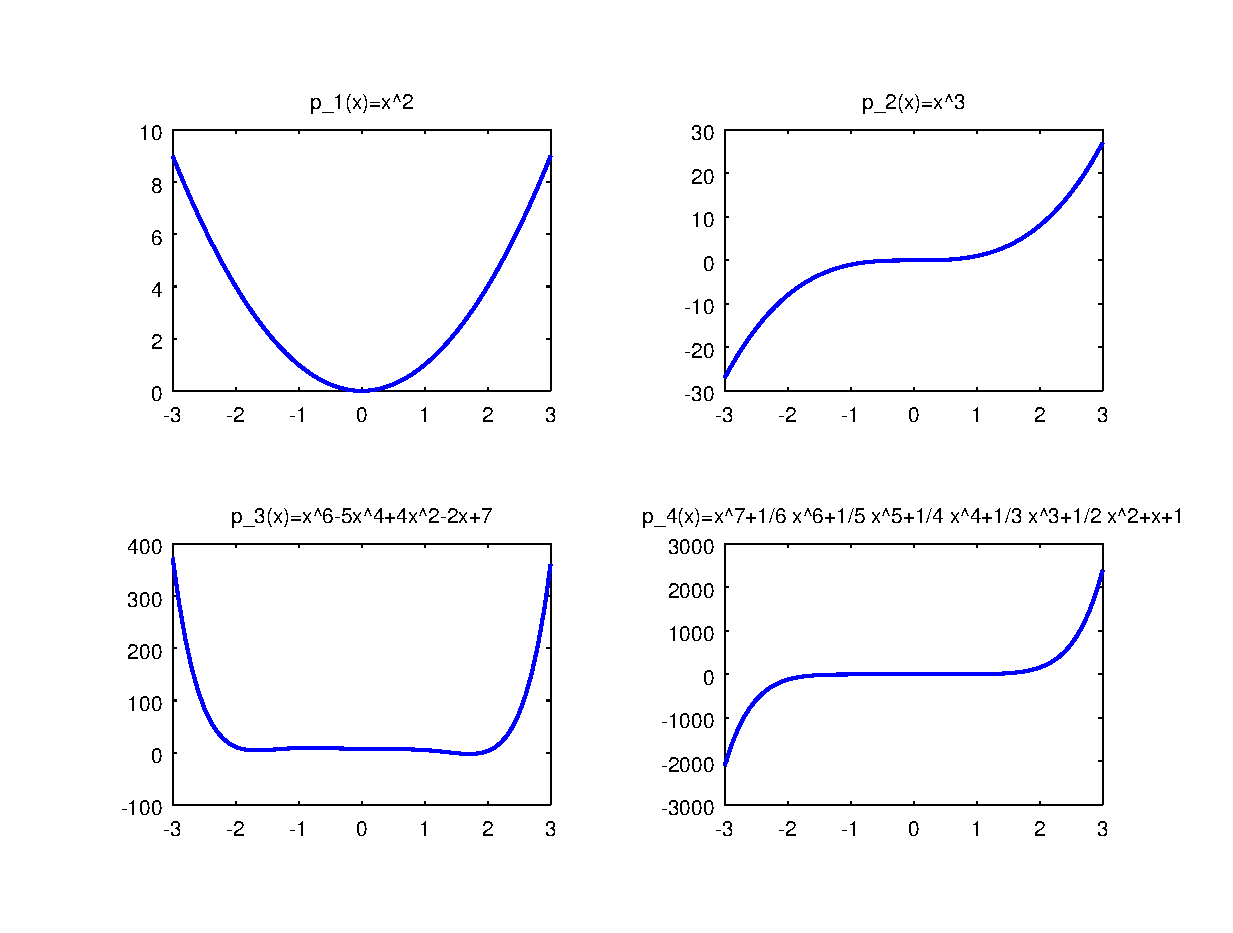
\includegraphics[scale=0.7]{grafpol.eps}
  \caption{Ejemplos de polinomios de una variable y coeficientes reales}
  \label{fig:polis}
  \end{figurebox}
\end{figure}
 
La importancia de los polinomios es altísima. ¿Te has preguntado alguna vez cómo calcula el $sen(15°)$ una calculadora o tu ordenador?, ¿cómo se detecta la huella de tu mano en una impresora? ¿Cómo se realizan predicciones de mercado? Pues en esto y muchísimo más están implicados los polinomios. Los polinomios tiene la bondad de que operarlos no es hacer otra cosas que sumas y multiplicaciones y tienen tan buenas propiedadess como continuidad, diferenciabilidad, $C^\infty$ que podemos aproximar funciones extrañísimas localmente por polinomios. Por ello vamos a dedicarles este número y el siguiente para que aprendan como usarlos en Octave y transversalmente aprendan algunas de sus aplicaciones. Diviértanse con ello. 

\section{Funciones de Octave que involucran polinomios}

Vamos a ver operaciones entre polinomios, evaluación de un polinomio, construcción de un polinomio a partir de sus raíces y el cálculo de las raíces de un polinomio.
\subsection{Operaciones entre polinomios}
Las operaciones suma y resta se realizarían con los comandos \textsl{+} y \textsl{-}. Por ejemplo probemos que queremos sumar el polinomio $p(x)=x^3+x^2+x+1$ con $q(x)=2x^2+2x$. ¿Cómo lo haríamos en Octave? Veamos el siguiente código:
\begin{octavebox}
\begin{verbatim}
 p=[1 1 1 1];
 q=[2 2 0]:
 s=p+q
\end{verbatim}
\end{octavebox}
Si lo has ejecutado te habrás encontrado con el siguiente error:

\textbf{operator +: nonconformant arguments (op1 is 1x4, op2 is 1x3)}. 

Si recuerdas bien en el número anterior vimos operaciones entre matrices y estamos representando un polinomio con una matriz, en particular un vector fila. Vimos que para sumar dos matrices estas deberían ser del mismo tamaño. Esa es la razón por la que no se ha realizado la operación correctamente. Lo corregimos, pues, en el siguiente código donde ya realizamos la operación resta también, ¿te ha coincidido con tus cuentas?
\begin{octavebox}
\begin{verbatim}
 p=[1 1 1 1];
 q=[0 2 2 0]:
 s=p+q
 r=p-q
\end{verbatim}
\end{octavebox}

Como sabemos dos polinomios de cualquier grado pueden ser multiplicados y además el resultado es un polinomio de grado la suma de los grados de los polinomios que se desean multiplicar. Para la multiplicación existe un comando que la realiza que es el comando \texttt{conv()}. Multipliquemos los polinomios $p(x)$ y $q(x)$ de antes.
\begin{octavebox}
\begin{verbatim}
 p=[1 1 1 1];
 q=[2 2 0];
 conv(p,q)
\end{verbatim}
\end{octavebox}

Dos polinomios también pueden ser divididos si el grado del dividendo es mayor o igual que el grado del divisor. El resultado de la operación nos da un cociente y un resto cuyo grado es menor que el del divisor. En Octave podemos realizar esta operación usando el comando \texttt{deconv()} y nos da dos salidas, el cociente y el resto. Damos un ejemplo en el siguiente código tomando como dividendo (D) el polinomio $p(x)$ y el divisor (d) el polinomio $q(x)$.
\begin{octavebox}
\begin{verbatim}
 D=[1 1 1 1];
 d=[2 2 0];
 [Q R]=deconv(p,q)
\end{verbatim}
\end{octavebox}
obteniendo como cociente el polinomio $\frac{1}{2}x$ y como resto el polinomio $x+1$.

\subsection{Evaluación de un polinomio y sus raíces}

Para evaluar un polinomio en un punto o en un conjunto de puntos usaremos el comando  \texttt{polyval(p,x)} donde  \texttt{p} será el polinomio a evaluar en notación Octave y  \texttt{x} un valor o una matriz de valores donde ser evaluado el polinomio. Ejecuta el siguiente código y observa los resultados.
\begin{octavebox}
\begin{verbatim}
 p=[1 2 3 4];
 polyval(p,0)
 polyval(p,1)
 polyval(p,[1 2 3;4 5 6])
\end{verbatim}
\end{octavebox}

El cálculo de las raíces de un polinomio $p(x)$ (esto son los puntos del eje x por donde el corta polinomio o más formalmente los valores $x$ tales que $p(x)=0$) no es un cálculo trivial. En la escuela nos enseñan como calcular las raíces de un polinomio de grado dos, pero a partir de grado tres el cómputo es mucho más complejo y además nos ponían ejemplos cuyas raíces eran enteras o como mucho racionales. Pero, esto parece un poco manipulado, ¿verdad? y bastante lejano a la realidad. El cálculo de raíces de un polinomio cualesquiera conlleva en la práctica un conjunto de conocimientos más sofisticados que involucran cálculo numérico. En un futuro podremos hablar un poco de ello. El comando de matlab que calcula, o más convenientemente dicho, que aproxima las raíces de un polinomio cualesquiera es el comando  \texttt{roots(\cdot)} , y los algoritmos que usa para el cálculo están actualizados constantemente según las mejoras de las investigaciones que se realizan para depurar todos esos algotitmos existentes.

Además tenemos el comando \texttt{poly(v)} que calcula un polinomio de grado mínimo y mónico (esto es, que el coeficiente director vale $1$) cuyas raíces son los elementos del vector $v$. Para ver como funcionan estos comandos ejecuta el siguiente código.

\begin{octavebox}
\begin{verbatim}
p=[1 2 3 4];
% Calculemos las raíces del polinomio p(x)
roots(p)
% Construyamos un polinomio cuyas raíces sean los elementos del vector fila v
v=[0 1 2 3 4]
t=poly(v)
% Calculemos sus raíces y comparemos con v, ¿son iguales?
roots(poly(v))
\end{verbatim}
\end{octavebox}


\section{Un reto: cálculo de un polinomio de grado tres}
En esta sección te proponemos un reto, escribir una función en Octave que realice lo siguiente: calcular los coeficientes del polinomio de grado tres que pase por cuatro puntos dados y que dibuje el polinomio resultante junto con los puntos dados. El output de la función serán los coeficientes y la figura. Mándanos tu programa y si eres el primero en tenerlo bien lo compartiremos con el resto en el próximo número y \textsl{recibirás un obsequio}.

Lo que esperamos es algo parecido a lo que se muestra en la Figura \ref{fig:pol3}.
\begin{figure}[ht!]
\begin{figurebox}
\begin{center}
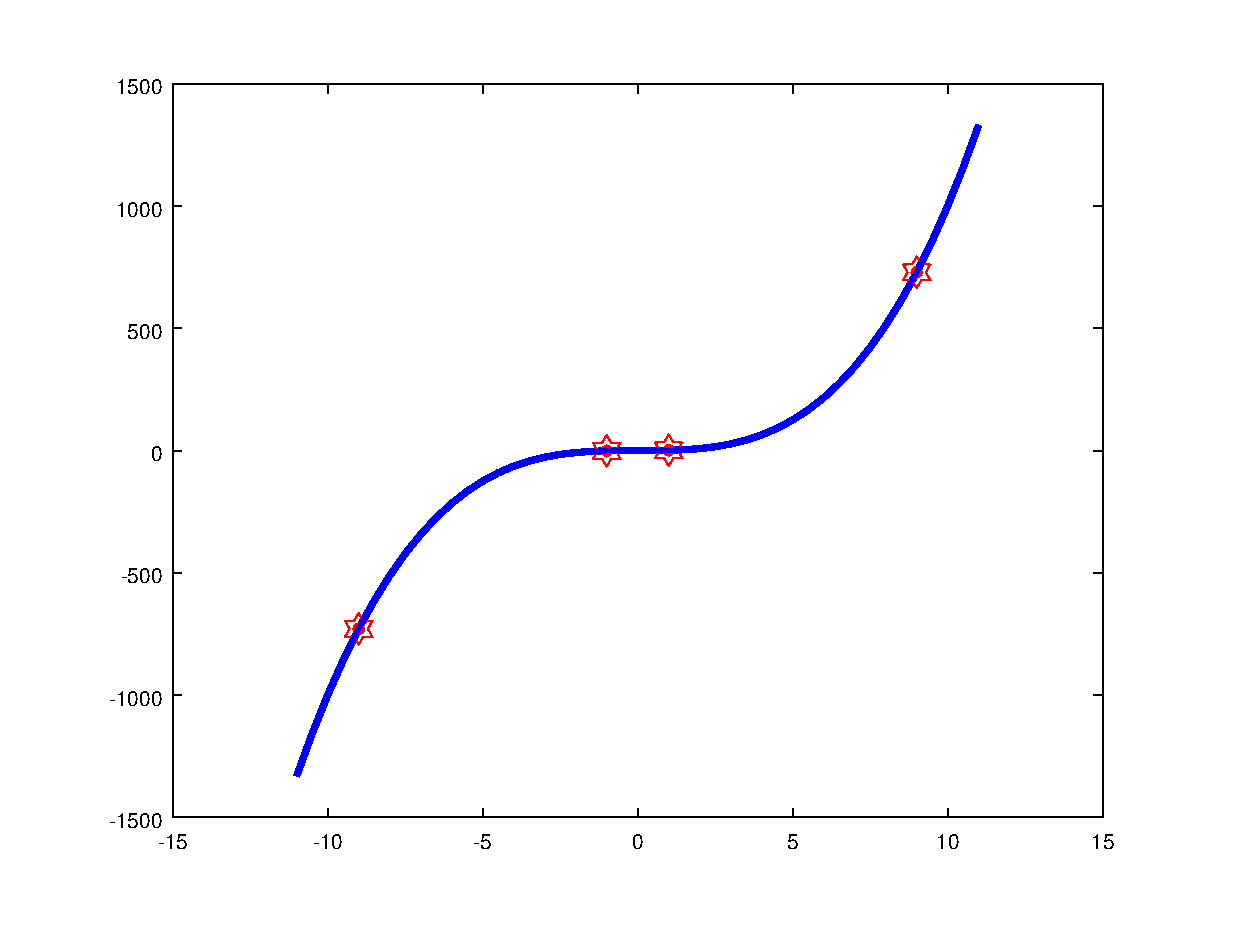
\includegraphics[scale=0.2]{polinomios3.eps}
\end{center}\caption{Polinomio calculado en azul, puntos dados en rojo}\label{fig:pol3}
\end{figurebox}
\end{figure}



\section{Programando: expresiones lógicas}
Según vayamos avanzando en la complejidad de los programas que vayamos desarrollando vamos a tener que hacer uso de expresiones lógicas, por ejemplo para incluirlas en expresiones condicionales. En la siguiente tabla mostramos la terminología a usar en las expresiones lógicas.

\begin{center}
\begin{tabular}{|cc||cc|}
\hline
$<$ & menor que & \&\& & Conjunción\\
\hline
$<=$ & menor o igual que & $||$ & Disyunción\\
\hline
$ >$ & mayor que & $\sim$ & Negación\\
\hline
$>=$ & mayor o igual que & xor & Disyunción exclusiva\\
\hline
$==$ & igual a & $\sim =$ & distinto de\\
\hline
\end{tabular}
\end{center}

Las expresiones lógicas dan como resultado booleanos: verdadero o falso. En Octave verdadero es representado con el dígito $1$ y falso con el dígito $0$.  Preuba el siguiente código.

\begin{octavebox}
\begin{verbatim}
x=2; y=3; z=4; A=[-3 0 3];
% Expresiones verdaderas

      x>0
      x+y>=z
      x==y-1
      x>0 && y<z
      x<0 || x>0
      A>=-3
      
% Expresiones falsas 

      xor(x>0,y>0)
      xor(x<0,y<0)
      ~(x>0)

\end{verbatim}
\end{octavebox}
  
Las expresiones lógicas pueden aparecer en expresiones condicionales (con el comando \textbf{if}) o expresiones de flujo de eventos (con los comandos \textbf{while} o \textbf{for}). Todas ellas las explicaremos con detalle en el siguiente número.
Intenta escribir un programa que dado un vector cuyo primer término es distinto de cero y por tanto representa un polinomio nos devuelva el grado de este. Te dejamos el codigo en el formato electrónico de la revista. No olvides chequearlo. Se llama \text{grado-pol.m}.

\vspace{3cm}
\noindent

\includegraphics[width=\textwidth]{pubmm.png}

\newpage
%%% Local Variables: 
%%% mode: latex
%%% TeX-master: "informaticaeningenieria"
%%% End: 





